\documentclass[a4paper,12pt]{article}
\usepackage[utf8x]{inputenc}
\usepackage[numbers,sort&compress]{natbib}
\usepackage{amsfonts}
\usepackage{amsthm}
\usepackage{fullpage}
\usepackage[pdftex]{graphicx}



\title{IRP Proposal}
\author{Pengfei Gao, s1144374}

\begin{document}

\maketitle

\begin{abstract}

In the recent days, the social networking media has been widely used by more and more people. There is a growing need to develop a powerful and efficient system tools to mining the useful and important information from the huge amount of data generated by users from those social networking media. The aim of this project is to develop such a real-time First Story Detection system to detect current hot events from the real-time stream of Twitter. The project will use Apache Distributed Stream Computing platform(S4) to process continuous unbounded streams of data and locality-sensitive hashing method to extract the features from the tweets.

\end{abstract}



\section{Purpose}


Twitter is a popular real-time information network that users can present and find the latest ideas, stories, news and opinions on what they interested. For example, when the news the pop star Michael Jackson's death came out, 22.64\% of the tweets posted contains the phrase "Michael Jackson", which enables the detection of the current hot events promptly.\newline



New event detection includes topic detection and tracking. A story is a topically cohesive segment of news that includes two or more declarative independent clauses about a single event. Given a sequence of stories, the goal of FSD is to identify the first story to discuss a particular event. In this context, an event is taken to be something that happens at some specific time and place, e.g., an earthquake striking the town of Sichuan in China, 2008.











\section{Background}



First Story Detection deals with spotting breaking news. For example, as soon as an earthquake happens, we want to know about it. We do not care about follow-up stories. Now, Twitter can be an excellent source of first stories and we have shown how they can be spotted using scalable algorithms based upon locality sensitive hashing. \newline


The traditional approach to detect the first story is using the vector space model which represents all the tweets as linearly-independent vectors and then projects them in some high-dimensional space. The coordinates of the space indicates the frequency of the particular words appeared in the tweets. Each new tweet is then compared to those existed ones and rank the similarities of those tweet vectors using dot product or cosine of the angle between vectors. If the new tweet’s similarity to the closet tweet is under a certain threshold, the new tweet is claimed to be a first story. This model is very popular in the topic detection and tracking area. \newline

Locality sensitive hashing (LSH) is a method of hashing input data and put the collision data into the same bucket. As the buckets size is much smaller than the total input data, the similar items will have high probability being put to the same bucket. When new tweet is hashed into a bucket, all the tweets in the same bucket will be compared and the most similar tweet will build a connection to the new one. 
\citep{Petrovic:2010} reports that simply using LSH for the closest neighbour search for the FSD performs poor and results in a high variance which a query point is hard to find the true nearest neighbour when it lies far away from all its neighbours. They introduce a modified LSH method which can reduce the variance and improve the accuracy. When the LSH approach claims a document is different from others, it will search through the inverted index of those existed documents with a limited number of the most recent document. This method works well and we will use it for this project. \newline



In the context of first story detection, we need to detect the current hot topic from the tweets that multiple users just update. The users may update their tweets at the same time. Therefore our FSD system should be distributed and scalable in order to track and analyze those users tweets at the same time. Although each tweet is just 140 character long, a user can tweet 100 or even more times a day. Especially some emergent important events happened such as Tunisian revolution, million people will tweet or retweet the corresponding news in the specific period of time. That leaves us a lot of tweets to track. However, we can not store all the tweets in the memory nor compare the new tweets to all the existed tweets. Thus, for an unbounded tweets streaming, the streaming FSD system should track each tweet and then make decisions whether the topic is seen before or a new one and then process the next tweet. The decision should be made in the limited time and space for each tweet. Such a system with all above features can be used to detect the first stories in the real time from an unbounded streaming of tweets from the Internet. \newline



As most of the first stories are just currently hot in a while and then being forgotten gradually, we need to limit the number of tweets in the bucket to a constant. We use a First-In-First-Out method here to keep the size of the bucket. In addition, we also limit the number of tweets to be compared when a new tweet comes. \citep{Petrovic:2010} compares each new tweet with less than 3L tweets which it collided with. \newline

People use Twitter to find the latest stories, ideas and news about what they interest in and also use it to express their opinions and share their daily life with their friends. In this sense, most of the tweets are not real stories but personal things, advertises and even spam. Therefore, simply using the FSD system to track and analyze every tweet will lead to an incredible number of new stories and most of this are not real first stories which we do not want. Our goal is to find the current significant first stories in the real time. To achieve this goal, \citep{Petrovic:2010} suggest a process that reduce the number of the non-important events. First they detect the a twitter’s nearest neighbour and assign a score to is using the cosine distance. They introduces a links relation to analyze threads of tweets: Tweet $a$ links to tweet $b$ if b is the nearest neighbour of a and $$d=1-cos(a,b)$$
where $t$ is a threshold defined by user. Then, for each tweet a, if $d<t$, they will assign $a$ to an existing thread containing the its nearest neighbour. Otherwise, they will create a new thread and $a$ will be first tweet for thread. As changing $t$ will affect on the granularity of threads, \citep{Petrovic:2010} find t belong to $[0.5,0.5]$ results are much better.\newline

Now we just need to compare the growing speed of those threads as a highest growing speed indicates the news of a new event is spreading widely and quickly. Thus, for each time interval we only capture the fastest growing thread and this thread represent the currently hottest first story. \newline











S4 , inspired by MapReduce, is a distributed processing system which spreads computation over a network of machines. It is a general-purpose, distributed, scalable, pluggable platform that used for processing continuous unbounded streams of data. Tasks communicate with each other via remote procedure calls using key-value pairs. Because of this, processing is scalable and fast. \newline



\citep{5693297} define a stream as a sequence of events in the form (K, A) where K is keys and A is the  attributes. S4 is designed to consume process such a stream. In S4, Events are arbitrary Java Objects that can be passed between PEs. Adapters convert the external incoming data streams into Events and then dispatched in named streams which identified by a key stream name. Then keyed data events are routed with affinity to Processing Elements (PEs), which consume the events and emit one or more events which may be consumed by other PEs, or publish results, possibly to an external data store or consumer.\newline

Processing Nodes (PNs) are the logical host to PEs which are responsible for listening to events, executing operations on the incoming events, dispatching events with the help of the communication layer, and emitting output events. Key-less PEs usually serve as entry point PEs: That is, the PEs that receive events from the outside world. This is because an adapter typically does not choose an S4 node based on a key in the event, but randomly (or in some other fashion that evenly distributes the events amongst the S4 nodes).\newline




\section{Methods}


We will define a PE type called TweetReceiverPE (PE1) which is configured to listen to the tweets stream. Each incoming tweet is event (I define Tweet object here) that has no key. So TweetReceiverPE is a keyless PE object that receives the new tweets and do some text preprocessing on Tweet object, such as tokenization, stemming, removing stop-words and some Twitter default charcters (i.e. @). After the preprocessing, each tweet is left with several important words. TweetReceiverPE will create a vector of these words representing this tweet and emit a new event of type TweetEvent, keyed on the hashes of these words vectors using LSH. TweetBucketPE objects listen for the TweetEvent events emited with key hash and put them into the corresponding buckets if their hashes are the same as the existed events in the bucket. For example, the TweetBucketPE object for key hash (PE2) receives all events of type TweetEvent keyed on hash. When a TweetEvent event for key comes, S4 looks up the TweetBucketPE object using the key hash. If the TweetBucketPE object is existed, The PE object is invoked and the TweetEvent will be saved into bucket. Otherwise a new TweetBucketPE object is created. Whenever a TweetBucketPE object saves an TweetEvent, it sends to updated information to the TweetSimilarityPE object. The key of the TweetSimilarityPE object is a random integer. Once TweetBucketPE object chooses a similarityID, it uses the similarityID in its whole lifecycle. The TweetBucketPE will calculate all the similarities for the new incoming TweetEvent object with other existed TweetEvent objects and find its nearest neighbour. When TweetBucketPE object has found the nearest neighbour of the new TweetEvent object, it sends a message including the TweetEvent object and its neighbour to the TweetThreadPE object. TweetThreadPE object checks whether the new TweetEvent object links to its nearest neighbour based on the Threading function mentioned in \cite{Petrovic:2010}: $$d=1-cos(a,b)$$
If the distance $d$ is smaller than the threshold $t$, the new Tweet will be assigned to an existing thread which its nearest neighbour belongs to. Otherwise, TweetThreadPE will create a new Thread object and the new Tweet will be its first tweet. The threshold t is set equal to $0.5$ according to \cite{Petrovic:2010}. \newline

	After the threads being updated, S4 will return the growing speed of each thread (simply the number of TweetEvent object each thread contains) and we are interested in those threads growing fastest. Therefore, in each time interval we just need to analysis the top fastest growing threads and these will be considered the first stories. 




\section{Evaluation}

-Details of the metrics by which you will evaluate the outcomes of your research; e.g., by comparing the output of your system with some gold standard, or with the ways in which humans perform a task, etc.


--you should probably identify some hypothesis you wish to test and
describe how you will go about testing it.  this will probably be
something like defining a baseline system of some kind (using S4 or
Storm for FSD), measuring it eg in terms of tweets per second
processed and then building a series of systems which explore the
relationship between the way S4 is used to solve the problem and
performance.  for example, what happens when you greatly increase the
rate that tweets arrive / PEs die etc.  so think of  interesting
questions to ask and say how you will solve them

--you also need to define a backup plan in case the main idea does not work.



\section{Outpus}



The output of this project will be a distributed real time software which detects the breaking news from Twitter. The software is implemented based on S4 framework.




\section{Workplan}

The final section identifies the workflow of my project along with expected completion dates. 

\begin{figure}[h]
\begin{center}
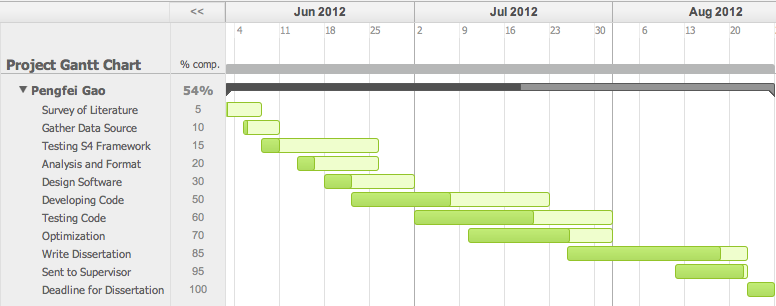
\includegraphics[scale=0.6]{gantt.png}
\end{center}
\end{figure}






\bibliographystyle{plain}
\bibliography{refs}


\end{document}
